\documentclass[a4paper,fleqn]{article} %Options in documentclass should be set to a4paper and fleqn.
\usepackage{modsim}
\usepackage{times}
\usepackage{natbib} %The three packages modsim, times and natbib are required.

\pagestyle{MODSIMheadings} %Calling the MODSIM Headings format
\MODSIMhead{Nervi et al. , Visualisation platform demo for experimental catchment data} %This is the content of the headings in all pages (except the first page). The format should be author, title of paper. If the title is too long, then use ... at the end. If more than two authors, then please use the "et al." format with et al. in italic, for example A. Author {\it et al.}, Title of the paper.

% Define any other command or required packages below:
%%%%%%%%%%%%%%%%%%%%%%%%%%%%%%%%%%%%%%%%%%%%%%%%%%%%%%%%%%%%%%%%%%%%%%%%%%%%%%%%%%%%%%%%%%%%%%%%%%%%%%%%%%%
\usepackage{rotating}
\usepackage{amsbsy,enumerate}
\usepackage{graphicx}
\usepackage{ccaption}
%\usepackage{academicons}
\usepackage{xcolor}
\usepackage[allbordercolors=white]{hyperref}
%\definecolor{orcidlogocol}{HTML}{A6CE39}
\setlength{\bibsep}{0.0pt}
\newcommand{\orcid}[1] {\hspace*{-1.5mm} \href{https://orcid.org/0000-0001-7867-7423}{
\includegraphics[scale=1.0]{orcid1.jpg}}}
%\newcommand{\orcid}[2] {\hspace*{-1.5mm} \href{https://orcid.org/2333}{
\includegraphics[scale=1.0]{orcid1.jpg}}}
\bibpunct{[}{]}{;}{a}{,}{,~}


% Text to appear in the header of the pages
\MODSIMhead{Nervi{\it et al.}, Visualisation platform demo for experimental catchment data}

\title{Visualisation platform demo for experimental catchment data
 } %title of your paper

\author{\underline{E. Nervi} %underline the presenter of the paper
 \address[A1]{\it{Instituto Nacional de Investigación Agropecuaria (INIA), FPTA 358,  Montevideo, Uruguay }} \orcid{0000-0000-0000-0000}, J. Alonso \address[B1]{\it{IMFIA, School of Engineering, Universidad de la República, Montevideo, Uruguay}}, W. Vervoort \address[C1]{\it{The University of Sydney, Sydney, Australia}},and W. Baetghen \addressmark[D1],\address[D1]{\it{IRI, The Earth Institute, Columbia University, New York, United States}}
}

\email{eliananervif@gmail.com}

\begin{document}

\begin{abstract}

South America has the highest proportion of forest plantations in the world, which also consists almost entirely of introduced species (\textit Eucalyptus spp. and \textit Pinus spp.). To promote sustainable forest management that adheres to the regulations for establishing new plantations and meets the standards required by international certifications, it is essential to generate local knowledge regarding the effects of forest plantations on natural resources. Using the paired catchment approach, Uruguay has implemented and maintains an operational network of small experimental catchments resulting from the partnership between government, academics, forest companies and national research programs, that has lasted for over 20 years. This monitoring program involves collecting and analyzing large amounts of data to understand how land use, rainfall and temperature affect water balance overtime. Even though time series of water quantity and quality can be used to monitor and understand these changes, it can be challenging to analyze and interpret them due to its size and complexity. The use of visualization tools can improve the understanding of the data, enabling the user to plot relationships between monitored variables and build interactive and customizable visualizations. RShiny is a web-based tool that allows users to to create a wide range of visualizations using the R programming. This versatile tool creates a visualization platform adaptable to other monitoring sites when the input data format is conserved. For technicians and researchers, this can help to identify data trends and evaluate correlations and relationships. Furthermore, visualization tools assists to communicate complex data to a wider audience, offering interactive and visually appealing plots that can help stakeholders and decision-makers understand the significance of the data and make informed decisions. In this work, a prototype of a visualization tool in RShiny was built to plot rainfall, flow and ET data for quality checks and analysis. The user can render dynamic time series plots and flow duration curves plots in the experimental catchment pair (treatment and control). In addition, it allows the user to do predefined quick analysis of the data, such as plotting flow differences between treatment and control catchment, displaying QQ and runoff coefficient plots. As a result, this platform provides the user with the ability to evaluate the response of a catchment to rainfall events, compare the hydrological behavior of two catchments and identify trends of the data.  We have tested this tool using local data from experimental small catchments in Uruguay (Figure 1). This demonstration showcased the potential of these tools for diverse future applications in analyzing experimental catchment data, which can be tailored to meet specific user requirements, leading to more informed decision making and improved management in water resources. 
\end{abstract}


\begin{figure}[b]
\centering
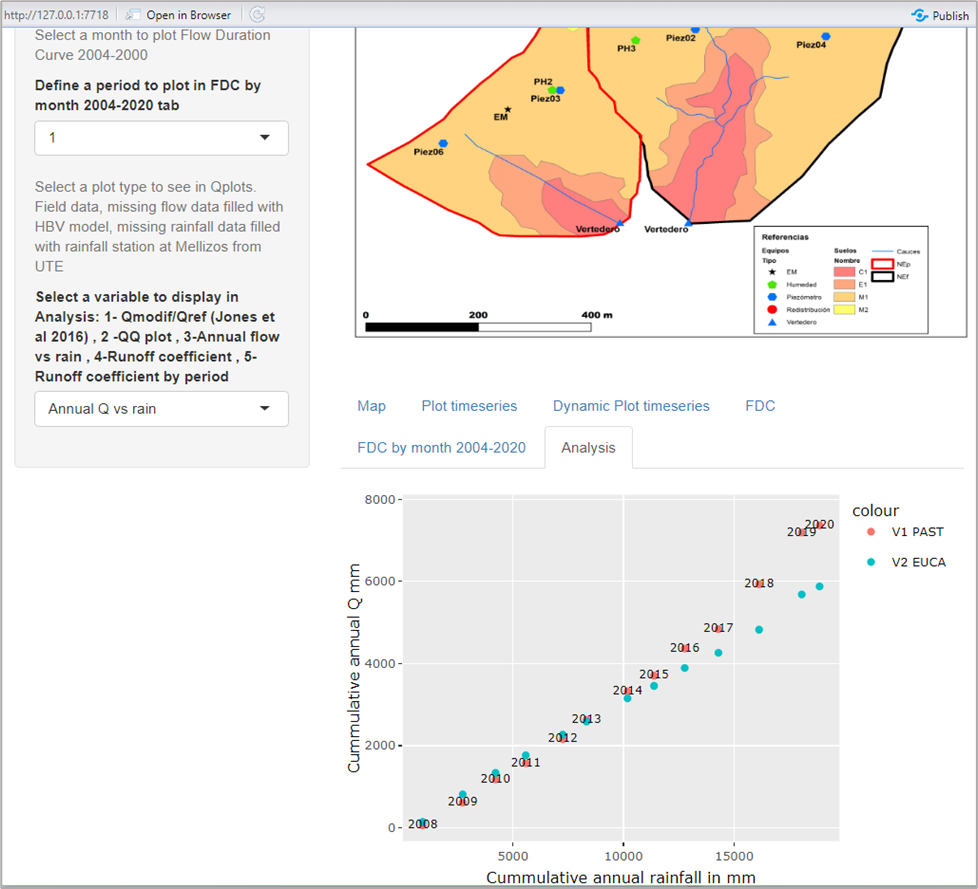
\includegraphics[width = 2cm,clip=true,scale = 0.3]{prototype_shiny.png}
\caption{Demo visualization of the tool web-page and analysis tab panel display of QQ plot in two experimental pasture and forested catchments in Río Negro, Uruguay.}
\end{figure}
\begin{keyword}
Data visualization, Pair catchment study, RShiny 
\end{keyword}

\maketitle


%%%%%%%%%%%%%%%%%%%%%%%%%%%%%%%%%%%%%%%%%%%%%%%%%%%%%%%%%%%%%%%%%
\bibliographystyle{agsm}
\bibliography{modsim}
%%%%%%%%%%%%%%%%%%%%%%%%%%%%%%%%%%%%%%%%%%%%%%%%%%%%%%%%%%%%%%%%%

	
\end{document}
